[TO DO: Add a section on missing values research]

The second hypothesis analyzes which environmental factors are the best predicters of temperature for Salt Lake City. According to the United States EPA ("EPA")\cite{epa_utah}, higher temperature results in either more or less percipitation and higher frequency of storms. This study performs a multiple linear regression of temperature against percipitation, number of thunderstorms per month, and minutes of sunlight per month. In conjuction with the EPA article noted above, we also considered two key characteristics when deciding which parameters we would inlcude in our study: (1) Linear relationship with temperature, and (2) Availability of data. For example, [TO CONFIRM WHY WE DID NOT INCLUDE, WHY DID WE NOT INCLUDE FOG? SEEMS PRETTY GOOD] we did not include total monthly snowfall or number of days with fog because they had a very weak linear realtionship (i.e. low R^2) with temperature, although we did have sufficient snowfall and number of days with fog data available. The parameter with the most significant linear relationship with temperature was, not suprisingly, minutes of sunlight. A major factor we had to consider here, however, was that sunlight data was only recorded from 1965 to 2004. Thus, in order to inlcude this parameter in our analysis, we needed to restrict our study down to this range (roughly 479 total months, or observations). Additionally, we limited our data used in our study to months in which we had available daya for all four parameters listed above. Therefore, when including temperature, percipation, and number of thunderstorms in our study, our sample size decreased from 479 months to 322 months because at least one of the these parameters was missing data for in the 479 months of data avialable between 1965 and 2004.

\begin{figure}
  \centering
  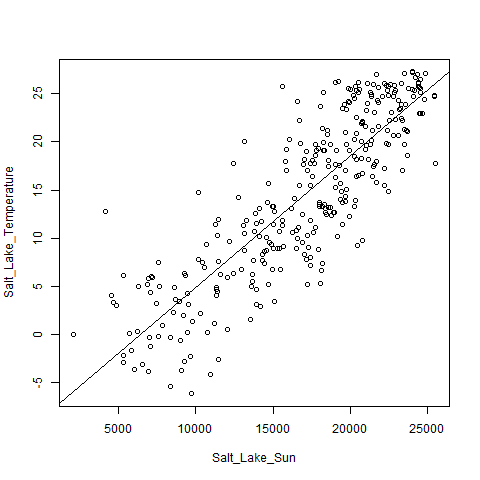
\includegraphics[width=15cm]{../data/img/Temp_vs_sun.PNG}
  \caption{Salt Lake City Temperature versus Sun}
  \label{fig:temp_vs_sun}
\end{figure}

\begin{figure}
  \centering
  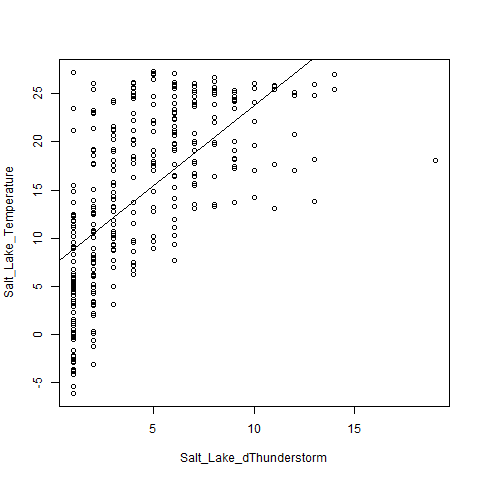
\includegraphics[width=15cm]{../data/img/Temp_vs_dThunderstorm.PNG}
  \caption{Salt Lake City Temperature versus Days of Thunderstorms}
  \label{fig:temp_vs_dthunderstorms}
\end{figure}

\begin{figure}
  \centering
  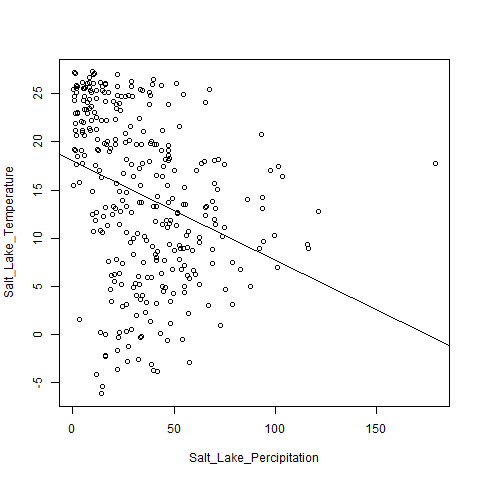
\includegraphics[width=15cm]{../data/img/Temp_vs_Percipitation.PNG}
  \caption{Salt Lake City Temperature versus Percipitation}
  \label{fig:temp_vs_percipitation}
\end{figure}

Turning specifically to our selected independent parameters, and as we conducted in our initial paramter selection process noted above, we compared temperature data by each independent variable, inlcuding a line of best fit. As expected, there is a strong positive correlation between minutes of sunlight and temperature, as seen in Figure \ref{fig:temp_vs_sun}. Similarly, albeit not as strong, there is also to be a positive correlation between number of thunderstorms and temperature, as seen in Figure \ref{fig:temp_vs_dthunderstorms}. Lastly, the correlation between percipitation and temperature is negative, as seen in Figure \ref{fig:temp_vs_percipitation}, which is expected in some regions as stated by the US EPA\cite{epa_utah}.

As an additional preliminarly analysis, in order to obtain a strong multiple linear regression model to estimate temperature, we sought to use parameters that are not highly correlated with each other, as including additional variables that are highly correlated is more likely to simply increase model complexity as opposed to imporve the model fit. Figure \ref{fig:correlation_plot}, which is a correlation matrix of the three independent parameters, suggests that the independent variables of sunlight, days of thunderstorm, and percipitation are not highly correlated, further supporting our decision to include them as parameters in our model.

\begin{figure}
  \centering
  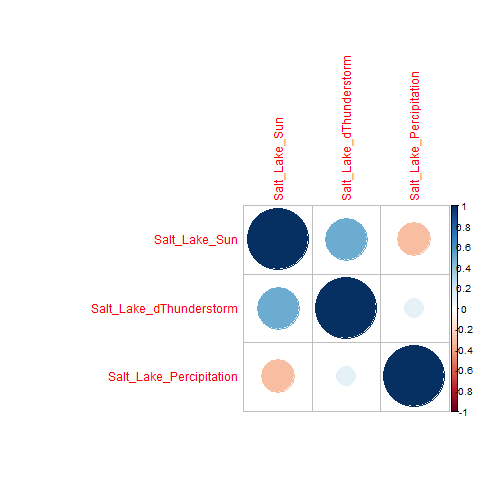
\includegraphics[width=10cm]{../data/img/correlation_plot.PNG}
  \caption{Correlation plot of chosen dependent variables}
  \label{fig:correlation_plot}
\end{figure}

[TO DO: NEED THE R OUTPUT FROM THE MULT LIN REG TO TALK ABOUT IT IN A PARAGRAPH] At this point, we conducted the analysis on the selected paramters. Per Figure [ADD TABLE OF SUMMARY FOR FIT OUTPUT], we can see the the model has an adjusted R^2 of ~80.0\%, meaning that roughly 80.0\% of the variance in temperature can be explained by the three predictors. Using the coefficients from the table, we may produce a formula for the fitted values, as seen in equation [ADD THE Y HAT EQUATION, Y_HAT = B_0 + X_1*B_1 + X_2*B_2 + X_3*B_3].

[WOULD WE LIKE TO INLCUDE A PARAGRAPH ON CONFIDENCE OR PREDICTION INTERVALS?]

Now that we have completed out multiple linear regression analysis on the three selected parameters, we turn to a final model comparison analysis. Here, we will conduct a best subset analysis to locate the best model at each model size, including 1, 2 and 3 parameters. After locating the best model at each parameter size, we will conduct a model comparison analysis, analyzing the adjusted R^2, AIC, and BIC values for each model.

The best subset selection process considers all 3 choose k [PUT IN MATH FORM] at each k number of parameters, k = 1, 2, 3. For each k, the best subset method will select the model with the lowest SSE. As can been seen in Figure [ADD FIGURE WITH *'S HERE], the best models for k = 1, 2, and 3 are sunlight, sunlihgt + days of thunderstorms, and sunlight + days of thunderstorms + percipation, respectively.

Now that we have our three best models at each k, we will calculate the following metrics for each model: (1) Adjusted R^2; (2) AIC; and, (3) BIC. The adjusted R^2 will show what percentage of the variance in the model is explained by the parameters, adjusting downward as model complexity increases. AIC and BIC are both penalized-likelihood criteria, where the BIC penalizes model compexity a bit more than AIC. Overall, the best model of the three will have the great adjusted R^2 and the lowest AIC and BIC values. As seen in Table [ADD TABLE OF THE VALUES HERE], the full model, or the one including all three independent paramters, is the best overall model to choose to estimate temperature.

\begin{table}[ht]
 \begin{centering}
 \begin{tabular}{|c|c c|} 
 \hline
 $$ & $\Delta T$ Salt Lake City & $\Delta T$ Rye Patch \\ [0.5ex] 
 \hline\hline
  $\mu$ & 1.1229 & 0.1317 \\ 
 \hline
 $\sigma$ & 1.9765 & 1.9226 \\
  \hline
 $n$ & 487 & 487 \\ 
  \hline
 $P_{Shapiro}$ & 0.0166 & 0.0003 \\ 
 \hline
 \end{tabular}
 \caption{Temperature Difference Statistics}
 \label{tab:lin_regression1}
 \end{centering}
\end{table}

\begin{table}[ht]
 \begin{centering}
 \begin{tabular}{|c|c|} 
 \hline
  $t$ & -16.46 \\ 
 \hline
 $df$ & 486 \\
  \hline
 $P$ & $2.2 \times 10^{-16}$ \\ 
  \hline
 Conf. Interval & $(-1.1095, -0.8728)$ \\ 
 \hline
 \end{tabular}
 \caption{Paired t Test Results for $\Delta T$}
 \label{tab:lin_regression2}
 \end{centering}
\end{table}